\documentclass[twoside]{book}

% Packages required by doxygen
\usepackage{fixltx2e}
\usepackage{calc}
\usepackage{doxygen}
\usepackage[export]{adjustbox} % also loads graphicx
\usepackage{graphicx}
\usepackage[utf8]{inputenc}
\usepackage{makeidx}
\usepackage{multicol}
\usepackage{multirow}
\PassOptionsToPackage{warn}{textcomp}
\usepackage{textcomp}
\usepackage[nointegrals]{wasysym}
\usepackage[table]{xcolor}

% NLS support packages
\usepackage[T2A]{fontenc}
\usepackage[russian]{babel}

% Font selection
\usepackage[T1]{fontenc}
\usepackage[scaled=.90]{helvet}
\usepackage{courier}
\usepackage{amssymb}
\usepackage{sectsty}
\renewcommand{\familydefault}{\sfdefault}
\allsectionsfont{%
  \fontseries{bc}\selectfont%
  \color{darkgray}%
}
\renewcommand{\DoxyLabelFont}{%
  \fontseries{bc}\selectfont%
  \color{darkgray}%
}
\newcommand{\+}{\discretionary{\mbox{\scriptsize$\hookleftarrow$}}{}{}}

% Page & text layout
\usepackage{geometry}
\geometry{%
  a4paper,%
  top=2.5cm,%
  bottom=2.5cm,%
  left=2.5cm,%
  right=2.5cm%
}
\tolerance=750
\hfuzz=15pt
\hbadness=750
\setlength{\emergencystretch}{15pt}
\setlength{\parindent}{0cm}
\setlength{\parskip}{3ex plus 2ex minus 2ex}
\makeatletter
\renewcommand{\paragraph}{%
  \@startsection{paragraph}{4}{0ex}{-1.0ex}{1.0ex}{%
    \normalfont\normalsize\bfseries\SS@parafont%
  }%
}
\renewcommand{\subparagraph}{%
  \@startsection{subparagraph}{5}{0ex}{-1.0ex}{1.0ex}{%
    \normalfont\normalsize\bfseries\SS@subparafont%
  }%
}
\makeatother

% Headers & footers
\usepackage{fancyhdr}
\pagestyle{fancyplain}
\fancyhead[LE]{\fancyplain{}{\bfseries\thepage}}
\fancyhead[CE]{\fancyplain{}{}}
\fancyhead[RE]{\fancyplain{}{\bfseries\leftmark}}
\fancyhead[LO]{\fancyplain{}{\bfseries\rightmark}}
\fancyhead[CO]{\fancyplain{}{}}
\fancyhead[RO]{\fancyplain{}{\bfseries\thepage}}
\fancyfoot[LE]{\fancyplain{}{}}
\fancyfoot[CE]{\fancyplain{}{}}
\fancyfoot[RE]{\fancyplain{}{\bfseries\scriptsize Создано системой Doxygen }}
\fancyfoot[LO]{\fancyplain{}{\bfseries\scriptsize Создано системой Doxygen }}
\fancyfoot[CO]{\fancyplain{}{}}
\fancyfoot[RO]{\fancyplain{}{}}
\renewcommand{\footrulewidth}{0.4pt}
\renewcommand{\chaptermark}[1]{%
  \markboth{#1}{}%
}
\renewcommand{\sectionmark}[1]{%
  \markright{\thesection\ #1}%
}

% Indices & bibliography
\usepackage{natbib}
\usepackage[titles]{tocloft}
\setcounter{tocdepth}{3}
\setcounter{secnumdepth}{5}
\makeindex

% Hyperlinks (required, but should be loaded last)
\usepackage{ifpdf}
\ifpdf
  \usepackage[pdftex,pagebackref=true]{hyperref}
\else
  \usepackage[ps2pdf,pagebackref=true]{hyperref}
\fi
\hypersetup{%
  colorlinks=true,%
  linkcolor=blue,%
  citecolor=blue,%
  unicode%
}

% Custom commands
\newcommand{\clearemptydoublepage}{%
  \newpage{\pagestyle{empty}\cleardoublepage}%
}

\usepackage{caption}
\captionsetup{labelsep=space,justification=centering,font={bf},singlelinecheck=off,skip=4pt,position=top}

%===== C O N T E N T S =====

\begin{document}

% Titlepage & ToC
\hypersetup{pageanchor=false,
             bookmarksnumbered=true,
             pdfencoding=unicode
            }
\pagenumbering{alph}
\begin{titlepage}
\vspace*{7cm}
\begin{center}%
{\Large Chess }\\
\vspace*{1cm}
{\large Создано системой Doxygen 1.8.14}\\
\end{center}
\end{titlepage}
\clearemptydoublepage
\pagenumbering{roman}
\tableofcontents
\clearemptydoublepage
\pagenumbering{arabic}
\hypersetup{pageanchor=true}

%--- Begin generated contents ---
\chapter{Иерархический список классов}
\section{Иерархия классов}
Иерархия классов.\begin{DoxyCompactList}
\item \contentsline{section}{Chess\+:\+:Clock}{\pageref{class_chess_1_1_clock}}{}
\item \contentsline{section}{Chess\+:\+:Game}{\pageref{class_chess_1_1_game}}{}
\item \contentsline{section}{Chess\+:\+:Game\+History}{\pageref{class_chess_1_1_game_history}}{}
\item \contentsline{section}{Chess\+:\+:Piece}{\pageref{class_chess_1_1_piece}}{}
\begin{DoxyCompactList}
\item \contentsline{section}{Chess\+:\+:Bishop}{\pageref{class_chess_1_1_bishop}}{}
\item \contentsline{section}{Chess\+:\+:King}{\pageref{class_chess_1_1_king}}{}
\item \contentsline{section}{Chess\+:\+:Knight}{\pageref{class_chess_1_1_knight}}{}
\item \contentsline{section}{Chess\+:\+:Pawn}{\pageref{class_chess_1_1_pawn}}{}
\item \contentsline{section}{Chess\+:\+:Queen}{\pageref{class_chess_1_1_queen}}{}
\item \contentsline{section}{Chess\+:\+:Rook}{\pageref{class_chess_1_1_rook}}{}
\end{DoxyCompactList}
\item \contentsline{section}{Chess\+:\+:Player}{\pageref{class_chess_1_1_player}}{}
\item \contentsline{section}{Chess\+:\+:Position}{\pageref{class_chess_1_1_position}}{}
\end{DoxyCompactList}

\chapter{Алфавитный указатель классов}
\section{Классы}
Классы с их кратким описанием.\begin{DoxyCompactList}
\item\contentsline{section}{\mbox{\hyperlink{class_chess_1_1_bishop}{Chess\+::\+Bishop}} }{\pageref{class_chess_1_1_bishop}}{}
\item\contentsline{section}{\mbox{\hyperlink{class_chess_1_1_clock}{Chess\+::\+Clock}} }{\pageref{class_chess_1_1_clock}}{}
\item\contentsline{section}{\mbox{\hyperlink{class_chess_1_1_game}{Chess\+::\+Game}} }{\pageref{class_chess_1_1_game}}{}
\item\contentsline{section}{\mbox{\hyperlink{class_chess_1_1_game_history}{Chess\+::\+Game\+History}} }{\pageref{class_chess_1_1_game_history}}{}
\item\contentsline{section}{\mbox{\hyperlink{class_chess_1_1_king}{Chess\+::\+King}} }{\pageref{class_chess_1_1_king}}{}
\item\contentsline{section}{\mbox{\hyperlink{class_chess_1_1_knight}{Chess\+::\+Knight}} }{\pageref{class_chess_1_1_knight}}{}
\item\contentsline{section}{\mbox{\hyperlink{class_chess_1_1_pawn}{Chess\+::\+Pawn}} }{\pageref{class_chess_1_1_pawn}}{}
\item\contentsline{section}{\mbox{\hyperlink{class_chess_1_1_piece}{Chess\+::\+Piece}} }{\pageref{class_chess_1_1_piece}}{}
\item\contentsline{section}{\mbox{\hyperlink{class_chess_1_1_player}{Chess\+::\+Player}} }{\pageref{class_chess_1_1_player}}{}
\item\contentsline{section}{\mbox{\hyperlink{class_chess_1_1_position}{Chess\+::\+Position}} }{\pageref{class_chess_1_1_position}}{}
\item\contentsline{section}{\mbox{\hyperlink{class_chess_1_1_queen}{Chess\+::\+Queen}} }{\pageref{class_chess_1_1_queen}}{}
\item\contentsline{section}{\mbox{\hyperlink{class_chess_1_1_rook}{Chess\+::\+Rook}} }{\pageref{class_chess_1_1_rook}}{}
\end{DoxyCompactList}

\chapter{Классы}
\hypertarget{class_chess_1_1_bishop}{}\section{Класс Chess\+:\+:Bishop}
\label{class_chess_1_1_bishop}\index{Chess\+::\+Bishop@{Chess\+::\+Bishop}}


Граф наследования\+:Chess\+:\+:Bishop\+:\nopagebreak
\begin{figure}[H]
\begin{center}
\leavevmode
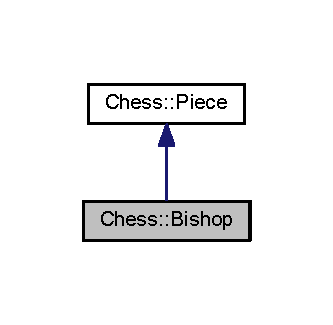
\includegraphics[width=160pt]{class_chess_1_1_bishop__inherit__graph}
\end{center}
\end{figure}


Граф связей класса Chess\+:\+:Bishop\+:\nopagebreak
\begin{figure}[H]
\begin{center}
\leavevmode
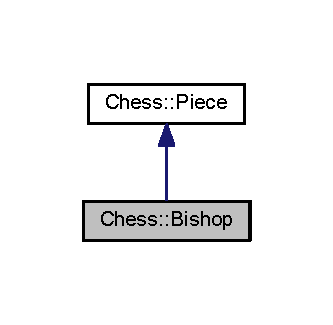
\includegraphics[width=160pt]{class_chess_1_1_bishop__coll__graph}
\end{center}
\end{figure}
\subsection*{Открытые члены}
\begin{DoxyCompactItemize}
\item 
\mbox{\Hypertarget{class_chess_1_1_bishop_a08f1b7e3e379c168958ab6819638d014}\label{class_chess_1_1_bishop_a08f1b7e3e379c168958ab6819638d014}} 
{\bfseries Bishop} (const Color color)
\item 
\mbox{\Hypertarget{class_chess_1_1_bishop_aafc2055191d4ba9df719ca8d35fd3a01}\label{class_chess_1_1_bishop_aafc2055191d4ba9df719ca8d35fd3a01}} 
bool {\bfseries check\+Move} (const \mbox{\hyperlink{class_chess_1_1_position}{Position}} \&pos\+\_\+current, const \mbox{\hyperlink{class_chess_1_1_position}{Position}} \&pos\+\_\+target, const std\+::array$<$ std\+::array$<$ \mbox{\hyperlink{class_chess_1_1_piece}{Piece}} $\ast$, B\+O\+A\+R\+D\+\_\+\+S\+I\+ZE $>$, B\+O\+A\+R\+D\+\_\+\+S\+I\+ZE $>$ \&chess\+\_\+board) const override
\item 
\mbox{\Hypertarget{class_chess_1_1_bishop_a235bab243b981b2d50f8694bbb9e2e77}\label{class_chess_1_1_bishop_a235bab243b981b2d50f8694bbb9e2e77}} 
\mbox{\hyperlink{class_chess_1_1_position}{Position}} $\ast$ {\bfseries return\+Available\+Moves} (int $\ast$list\+\_\+len, const \mbox{\hyperlink{class_chess_1_1_position}{Position}} \&pos\+\_\+current, const std\+::array$<$ std\+::array$<$ \mbox{\hyperlink{class_chess_1_1_piece}{Piece}} $\ast$, B\+O\+A\+R\+D\+\_\+\+S\+I\+ZE $>$, B\+O\+A\+R\+D\+\_\+\+S\+I\+ZE $>$ \&chess\+\_\+board) const override
\item 
\mbox{\Hypertarget{class_chess_1_1_bishop_acad16beae041ce1e7d34b2cac9d6d0f9}\label{class_chess_1_1_bishop_acad16beae041ce1e7d34b2cac9d6d0f9}} 
bool {\bfseries check\+Reachability} (const \mbox{\hyperlink{class_chess_1_1_position}{Position}} \&pos\+\_\+current, const \mbox{\hyperlink{class_chess_1_1_position}{Position}} \&pos\+\_\+target, const std\+::array$<$ std\+::array$<$ \mbox{\hyperlink{class_chess_1_1_piece}{Piece}} $\ast$, B\+O\+A\+R\+D\+\_\+\+S\+I\+ZE $>$, B\+O\+A\+R\+D\+\_\+\+S\+I\+ZE $>$ \&chess\+\_\+board) const override
\end{DoxyCompactItemize}
\subsection*{Дополнительные унаследованные члены}


Объявления и описания членов классов находятся в файлах\+:\begin{DoxyCompactItemize}
\item 
Pieces/bishop.\+h\item 
Pieces/bishop.\+cpp\end{DoxyCompactItemize}

\hypertarget{class_chess_1_1_clock}{}\section{Класс Chess\+:\+:Clock}
\label{class_chess_1_1_clock}\index{Chess\+::\+Clock@{Chess\+::\+Clock}}
\subsection*{Открытые типы}
\begin{DoxyCompactItemize}
\item 
\mbox{\Hypertarget{class_chess_1_1_clock_a043cae508eb20b95269121cf2a242fb5}\label{class_chess_1_1_clock_a043cae508eb20b95269121cf2a242fb5}} 
enum {\bfseries Player\+Color} \{ {\bfseries P\+L\+A\+Y\+E\+R\+\_\+\+W\+H\+I\+TE} = 1, 
{\bfseries P\+L\+A\+Y\+E\+R\+\_\+\+B\+L\+A\+CK}
 \}
\end{DoxyCompactItemize}
\subsection*{Открытые члены}
\begin{DoxyCompactItemize}
\item 
\mbox{\Hypertarget{class_chess_1_1_clock_adac346380d40d59ac4c12fde8176ea58}\label{class_chess_1_1_clock_adac346380d40d59ac4c12fde8176ea58}} 
void {\bfseries set\+Time\+Sec} (const long long time, const Player\+Color player\+\_\+color)
\item 
\mbox{\Hypertarget{class_chess_1_1_clock_a9d724505115b54ccca5832d3dddc9570}\label{class_chess_1_1_clock_a9d724505115b54ccca5832d3dddc9570}} 
\mbox{\hyperlink{class_chess_1_1_clock}{Clock}} \& {\bfseries add\+Time\+Sec} (const long long value, const Player\+Color player\+\_\+color)
\item 
\mbox{\Hypertarget{class_chess_1_1_clock_ab113c85d844a690807d096c3a84244c8}\label{class_chess_1_1_clock_ab113c85d844a690807d096c3a84244c8}} 
long long {\bfseries get\+Time\+Sec} (const Player\+Color player\+\_\+color) const
\item 
\mbox{\Hypertarget{class_chess_1_1_clock_a94c24e8e2d7c53bcfa880d9201268332}\label{class_chess_1_1_clock_a94c24e8e2d7c53bcfa880d9201268332}} 
void {\bfseries print\+Time} (std\+::ostream \&os, const Player\+Color player\+\_\+color) const
\item 
\mbox{\Hypertarget{class_chess_1_1_clock_a0ab5423b0a997aa13d7b6131c46d1358}\label{class_chess_1_1_clock_a0ab5423b0a997aa13d7b6131c46d1358}} 
void {\bfseries reset} ()
\end{DoxyCompactItemize}


Объявления и описания членов классов находятся в файлах\+:\begin{DoxyCompactItemize}
\item 
clock.\+h\item 
clock.\+cpp\end{DoxyCompactItemize}

\hypertarget{class_chess_1_1_game}{}\section{Класс Chess\+:\+:Game}
\label{class_chess_1_1_game}\index{Chess\+::\+Game@{Chess\+::\+Game}}
\subsection*{Открытые типы}
\begin{DoxyCompactItemize}
\item 
\mbox{\Hypertarget{class_chess_1_1_game_a46c61f3f01bbe9e153de2d0fb17be7a3}\label{class_chess_1_1_game_a46c61f3f01bbe9e153de2d0fb17be7a3}} 
enum {\bfseries Game\+Status} \{ {\bfseries N\+O\+\_\+\+G\+A\+ME}, 
{\bfseries G\+A\+M\+E\+\_\+\+ON}, 
{\bfseries G\+A\+M\+E\+\_\+\+O\+V\+ER}
 \}
\item 
\mbox{\Hypertarget{class_chess_1_1_game_acf87322c373bb63671b87c5a6b68129d}\label{class_chess_1_1_game_acf87322c373bb63671b87c5a6b68129d}} 
enum {\bfseries Current\+Game\+Status} \{ {\bfseries N\+O\+T\+H\+I\+NG}, 
{\bfseries C\+H\+E\+CK}, 
{\bfseries M\+A\+TE}, 
{\bfseries S\+T\+A\+L\+E\+\_\+\+M\+A\+TE}
 \}
\end{DoxyCompactItemize}
\subsection*{Открытые члены}
\begin{DoxyCompactItemize}
\item 
\mbox{\Hypertarget{class_chess_1_1_game_aec4cf66335f57f6a5f655b750e57e0fa}\label{class_chess_1_1_game_aec4cf66335f57f6a5f655b750e57e0fa}} 
void {\bfseries set\+Players\+Names} (const char $\ast$player\+\_\+white\+\_\+name, const char $\ast$player\+\_\+black\+\_\+name)
\item 
\mbox{\Hypertarget{class_chess_1_1_game_a4efb0d8ba450f51a480afc1e191cc66a}\label{class_chess_1_1_game_a4efb0d8ba450f51a480afc1e191cc66a}} 
const char $\ast$ {\bfseries get\+Player\+Name} (const Piece\+::\+Color player\+\_\+color) const
\item 
\mbox{\Hypertarget{class_chess_1_1_game_a8cab7920c359cf67801ac3fd587fa3d7}\label{class_chess_1_1_game_a8cab7920c359cf67801ac3fd587fa3d7}} 
Piece\+::\+Color {\bfseries get\+Active\+Player\+Color} () const
\item 
\mbox{\Hypertarget{class_chess_1_1_game_a89c89d64fc10d4fd559491f9de98a8a9}\label{class_chess_1_1_game_a89c89d64fc10d4fd559491f9de98a8a9}} 
void {\bfseries print\+Board} (std\+::ostream \&os) const
\item 
\mbox{\Hypertarget{class_chess_1_1_game_ae8638ccdb0ef3bf39a6affa30aa1258f}\label{class_chess_1_1_game_ae8638ccdb0ef3bf39a6affa30aa1258f}} 
void {\bfseries start\+Game} ()
\item 
\mbox{\Hypertarget{class_chess_1_1_game_a46f78f45e092de4878600e290640d38b}\label{class_chess_1_1_game_a46f78f45e092de4878600e290640d38b}} 
Game\+Status {\bfseries get\+Game\+Status} () const
\item 
\mbox{\Hypertarget{class_chess_1_1_game_a5403d6708175f73d8249990f4cdb91eb}\label{class_chess_1_1_game_a5403d6708175f73d8249990f4cdb91eb}} 
Current\+Game\+Status {\bfseries get\+Current\+Game\+Status} () const
\item 
\mbox{\Hypertarget{class_chess_1_1_game_af8d2110ad5a08a88cab48c52be58fe42}\label{class_chess_1_1_game_af8d2110ad5a08a88cab48c52be58fe42}} 
bool {\bfseries make\+Move} (const char file\+\_\+current, const int rank\+\_\+current, const char file\+\_\+target, const int rank\+\_\+target)
\item 
\mbox{\Hypertarget{class_chess_1_1_game_aae5ab8b7d4591c466abd8d53f453415b}\label{class_chess_1_1_game_aae5ab8b7d4591c466abd8d53f453415b}} 
bool {\bfseries make\+Move} (const int x1, const int y1, const int x2, const int y2)
\item 
\mbox{\Hypertarget{class_chess_1_1_game_ad41f5a27992a255dfda146b2955b2b08}\label{class_chess_1_1_game_ad41f5a27992a255dfda146b2955b2b08}} 
bool {\bfseries make\+Move} (const \mbox{\hyperlink{class_chess_1_1_position}{Position}} \&pos\+\_\+current, const \mbox{\hyperlink{class_chess_1_1_position}{Position}} \&pos\+\_\+target)
\item 
\mbox{\Hypertarget{class_chess_1_1_game_a76a66b4e73ba5086b587dac9b5539840}\label{class_chess_1_1_game_a76a66b4e73ba5086b587dac9b5539840}} 
void {\bfseries add\+Time\+To\+Previous\+Player} (const long long time\+\_\+sec)
\item 
\mbox{\Hypertarget{class_chess_1_1_game_ade1027e22302d19ac285fec5a0a3d4c5}\label{class_chess_1_1_game_ade1027e22302d19ac285fec5a0a3d4c5}} 
void {\bfseries print\+History} (std\+::ostream \&os) const
\end{DoxyCompactItemize}


Объявления и описания членов классов находятся в файлах\+:\begin{DoxyCompactItemize}
\item 
game.\+h\item 
game.\+cpp\end{DoxyCompactItemize}

\hypertarget{class_chess_1_1_game_history}{}\section{Класс Chess\+:\+:Game\+History}
\label{class_chess_1_1_game_history}\index{Chess\+::\+Game\+History@{Chess\+::\+Game\+History}}
\subsection*{Открытые типы}
\begin{DoxyCompactItemize}
\item 
\mbox{\Hypertarget{class_chess_1_1_game_history_a1e66f8172e7db7d2f05a5b8c87d1ba0f}\label{class_chess_1_1_game_history_a1e66f8172e7db7d2f05a5b8c87d1ba0f}} 
enum {\bfseries Move\+Status} \{ {\bfseries N\+O\+\_\+\+M\+O\+VE}, 
{\bfseries M\+O\+V\+E\+\_\+\+D\+O\+NE}, 
{\bfseries T\+A\+K\+E\+N\+\_\+\+E\+N\+E\+M\+Y\+\_\+\+P\+I\+E\+CE}
 \}
\end{DoxyCompactItemize}
\subsection*{Открытые члены}
\begin{DoxyCompactItemize}
\item 
\mbox{\Hypertarget{class_chess_1_1_game_history_a04ae57210f35d767c974e5ef98756c3b}\label{class_chess_1_1_game_history_a04ae57210f35d767c974e5ef98756c3b}} 
\mbox{\hyperlink{class_chess_1_1_game_history}{Game\+History}} \& {\bfseries add\+Move\+To\+History} (const char $\ast$move)
\item 
\mbox{\Hypertarget{class_chess_1_1_game_history_a6f9576ffb5086eb9706ea88e788cc0d6}\label{class_chess_1_1_game_history_a6f9576ffb5086eb9706ea88e788cc0d6}} 
\mbox{\hyperlink{class_chess_1_1_game_history}{Game\+History}} \& {\bfseries add\+Move\+To\+History} (const \mbox{\hyperlink{class_chess_1_1_position}{Position}} \&pos\+\_\+current, const \mbox{\hyperlink{class_chess_1_1_position}{Position}} \&pos\+\_\+target, const Piece\+::\+Name piece\+\_\+name, const Move\+Status move\+\_\+status, const Piece\+::\+Name piece\+\_\+name\+\_\+new, const int move\+\_\+result)
\item 
\mbox{\Hypertarget{class_chess_1_1_game_history_aafb9294b1c8cfdaad4603c900ddc00aa}\label{class_chess_1_1_game_history_aafb9294b1c8cfdaad4603c900ddc00aa}} 
\mbox{\hyperlink{class_chess_1_1_game_history}{Game\+History}} \& {\bfseries append\+To\+Last\+Move} (const \mbox{\hyperlink{class_chess_1_1_position}{Position}} \&pos\+\_\+current, const \mbox{\hyperlink{class_chess_1_1_position}{Position}} \&pos\+\_\+target, const Piece\+::\+Name piece\+\_\+name, const Move\+Status move\+\_\+status, const Piece\+::\+Name piece\+\_\+name\+\_\+new, const int move\+\_\+result)
\item 
\mbox{\Hypertarget{class_chess_1_1_game_history_ab774acd3d1b1fa6185e567d2fcebb41f}\label{class_chess_1_1_game_history_ab774acd3d1b1fa6185e567d2fcebb41f}} 
\mbox{\hyperlink{class_chess_1_1_game_history}{Game\+History}} \& {\bfseries delete\+Last\+Move} ()
\item 
\mbox{\Hypertarget{class_chess_1_1_game_history_ac55b4d4260cf19775c3263ef41b73500}\label{class_chess_1_1_game_history_ac55b4d4260cf19775c3263ef41b73500}} 
const char $\ast$ {\bfseries return\+As\+String} () const
\item 
\mbox{\Hypertarget{class_chess_1_1_game_history_a4270ac251625e361794ac2f3ceb1dd1f}\label{class_chess_1_1_game_history_a4270ac251625e361794ac2f3ceb1dd1f}} 
void {\bfseries clear\+History} ()
\item 
\mbox{\Hypertarget{class_chess_1_1_game_history_a3fb2cf5a5c699684da9e8cd1e2277c79}\label{class_chess_1_1_game_history_a3fb2cf5a5c699684da9e8cd1e2277c79}} 
void {\bfseries print\+History} (std\+::ostream \&os) const
\end{DoxyCompactItemize}


Объявления и описания членов классов находятся в файлах\+:\begin{DoxyCompactItemize}
\item 
gamehistory.\+h\item 
gamehistory.\+cpp\end{DoxyCompactItemize}

\hypertarget{class_chess_1_1_king}{}\section{Класс Chess\+:\+:King}
\label{class_chess_1_1_king}\index{Chess\+::\+King@{Chess\+::\+King}}


Граф наследования\+:Chess\+:\+:King\+:\nopagebreak
\begin{figure}[H]
\begin{center}
\leavevmode
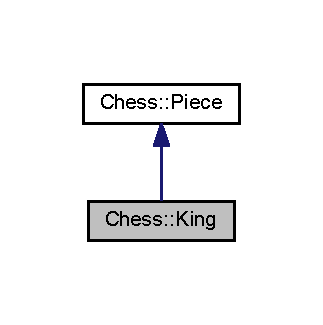
\includegraphics[width=155pt]{class_chess_1_1_king__inherit__graph}
\end{center}
\end{figure}


Граф связей класса Chess\+:\+:King\+:\nopagebreak
\begin{figure}[H]
\begin{center}
\leavevmode
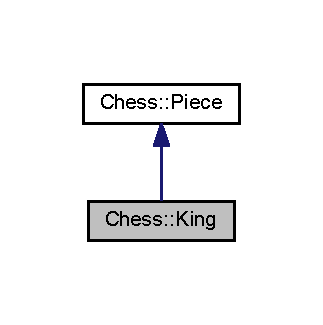
\includegraphics[width=155pt]{class_chess_1_1_king__coll__graph}
\end{center}
\end{figure}
\subsection*{Открытые члены}
\begin{DoxyCompactItemize}
\item 
\mbox{\Hypertarget{class_chess_1_1_king_a66db2fe8f54a001bd181591cdccba958}\label{class_chess_1_1_king_a66db2fe8f54a001bd181591cdccba958}} 
{\bfseries King} (const Color color)
\item 
\mbox{\Hypertarget{class_chess_1_1_king_a2a99eca45d27801a80eaded7aee690cb}\label{class_chess_1_1_king_a2a99eca45d27801a80eaded7aee690cb}} 
bool {\bfseries check\+Move} (const \mbox{\hyperlink{class_chess_1_1_position}{Position}} \&pos\+\_\+current, const \mbox{\hyperlink{class_chess_1_1_position}{Position}} \&pos\+\_\+target, const std\+::array$<$ std\+::array$<$ \mbox{\hyperlink{class_chess_1_1_piece}{Piece}} $\ast$, B\+O\+A\+R\+D\+\_\+\+S\+I\+ZE $>$, B\+O\+A\+R\+D\+\_\+\+S\+I\+ZE $>$ \&chess\+\_\+board) const override
\item 
\mbox{\Hypertarget{class_chess_1_1_king_a07ef876e1c3196200042cacccfd33cbb}\label{class_chess_1_1_king_a07ef876e1c3196200042cacccfd33cbb}} 
\mbox{\hyperlink{class_chess_1_1_position}{Position}} $\ast$ {\bfseries return\+Available\+Moves} (int $\ast$list\+\_\+len, const \mbox{\hyperlink{class_chess_1_1_position}{Position}} \&pos\+\_\+current, const std\+::array$<$ std\+::array$<$ \mbox{\hyperlink{class_chess_1_1_piece}{Piece}} $\ast$, B\+O\+A\+R\+D\+\_\+\+S\+I\+ZE $>$, B\+O\+A\+R\+D\+\_\+\+S\+I\+ZE $>$ \&chess\+\_\+board) const override
\item 
\mbox{\Hypertarget{class_chess_1_1_king_a986c2dd316a9daec8714a773fa575d79}\label{class_chess_1_1_king_a986c2dd316a9daec8714a773fa575d79}} 
bool {\bfseries check\+Reachability} (const \mbox{\hyperlink{class_chess_1_1_position}{Position}} \&pos\+\_\+current, const \mbox{\hyperlink{class_chess_1_1_position}{Position}} \&pos\+\_\+target, const std\+::array$<$ std\+::array$<$ \mbox{\hyperlink{class_chess_1_1_piece}{Piece}} $\ast$, B\+O\+A\+R\+D\+\_\+\+S\+I\+ZE $>$, B\+O\+A\+R\+D\+\_\+\+S\+I\+ZE $>$ \&chess\+\_\+board) const override
\end{DoxyCompactItemize}
\subsection*{Дополнительные унаследованные члены}


Объявления и описания членов классов находятся в файлах\+:\begin{DoxyCompactItemize}
\item 
Pieces/king.\+h\item 
Pieces/king.\+cpp\end{DoxyCompactItemize}

\hypertarget{class_chess_1_1_knight}{}\section{Класс Chess\+:\+:Knight}
\label{class_chess_1_1_knight}\index{Chess\+::\+Knight@{Chess\+::\+Knight}}


Граф наследования\+:Chess\+:\+:Knight\+:\nopagebreak
\begin{figure}[H]
\begin{center}
\leavevmode
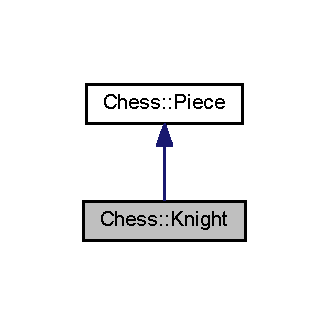
\includegraphics[width=158pt]{class_chess_1_1_knight__inherit__graph}
\end{center}
\end{figure}


Граф связей класса Chess\+:\+:Knight\+:\nopagebreak
\begin{figure}[H]
\begin{center}
\leavevmode
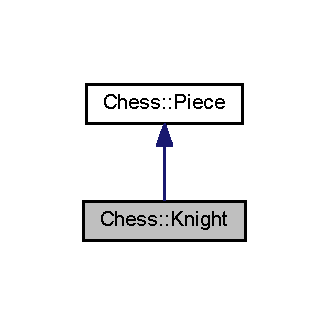
\includegraphics[width=158pt]{class_chess_1_1_knight__coll__graph}
\end{center}
\end{figure}
\subsection*{Открытые члены}
\begin{DoxyCompactItemize}
\item 
\mbox{\Hypertarget{class_chess_1_1_knight_a74ada3d5ae9ac1b5ae259ceba34289dd}\label{class_chess_1_1_knight_a74ada3d5ae9ac1b5ae259ceba34289dd}} 
{\bfseries Knight} (const Color color)
\item 
\mbox{\Hypertarget{class_chess_1_1_knight_a56ce2d3c2ee43f9bbb7a2de40dd294c3}\label{class_chess_1_1_knight_a56ce2d3c2ee43f9bbb7a2de40dd294c3}} 
bool {\bfseries check\+Move} (const \mbox{\hyperlink{class_chess_1_1_position}{Position}} \&pos\+\_\+current, const \mbox{\hyperlink{class_chess_1_1_position}{Position}} \&pos\+\_\+target, const std\+::array$<$ std\+::array$<$ \mbox{\hyperlink{class_chess_1_1_piece}{Piece}} $\ast$, B\+O\+A\+R\+D\+\_\+\+S\+I\+ZE $>$, B\+O\+A\+R\+D\+\_\+\+S\+I\+ZE $>$ \&chess\+\_\+board) const override
\item 
\mbox{\Hypertarget{class_chess_1_1_knight_af52d6ea731a3615a6d6e1c0a5985e1ad}\label{class_chess_1_1_knight_af52d6ea731a3615a6d6e1c0a5985e1ad}} 
\mbox{\hyperlink{class_chess_1_1_position}{Position}} $\ast$ {\bfseries return\+Available\+Moves} (int $\ast$list\+\_\+len, const \mbox{\hyperlink{class_chess_1_1_position}{Position}} \&pos\+\_\+current, const std\+::array$<$ std\+::array$<$ \mbox{\hyperlink{class_chess_1_1_piece}{Piece}} $\ast$, B\+O\+A\+R\+D\+\_\+\+S\+I\+ZE $>$, B\+O\+A\+R\+D\+\_\+\+S\+I\+ZE $>$ \&chess\+\_\+board) const override
\item 
\mbox{\Hypertarget{class_chess_1_1_knight_a2cd473555390e4cb9e5f0ac0594e91f2}\label{class_chess_1_1_knight_a2cd473555390e4cb9e5f0ac0594e91f2}} 
bool {\bfseries check\+Reachability} (const \mbox{\hyperlink{class_chess_1_1_position}{Position}} \&pos\+\_\+current, const \mbox{\hyperlink{class_chess_1_1_position}{Position}} \&pos\+\_\+target, const std\+::array$<$ std\+::array$<$ \mbox{\hyperlink{class_chess_1_1_piece}{Piece}} $\ast$, B\+O\+A\+R\+D\+\_\+\+S\+I\+ZE $>$, B\+O\+A\+R\+D\+\_\+\+S\+I\+ZE $>$ \&chess\+\_\+board) const override
\end{DoxyCompactItemize}
\subsection*{Дополнительные унаследованные члены}


Объявления и описания членов классов находятся в файлах\+:\begin{DoxyCompactItemize}
\item 
Pieces/knight.\+h\item 
Pieces/knight.\+cpp\end{DoxyCompactItemize}

\hypertarget{class_chess_1_1_pawn}{}\section{Класс Chess\+:\+:Pawn}
\label{class_chess_1_1_pawn}\index{Chess\+::\+Pawn@{Chess\+::\+Pawn}}


Граф наследования\+:Chess\+:\+:Pawn\+:\nopagebreak
\begin{figure}[H]
\begin{center}
\leavevmode
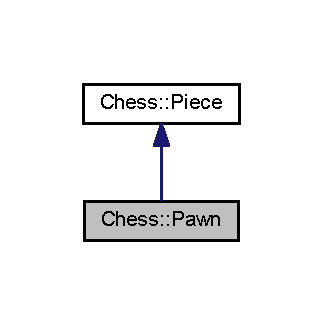
\includegraphics[width=155pt]{class_chess_1_1_pawn__inherit__graph}
\end{center}
\end{figure}


Граф связей класса Chess\+:\+:Pawn\+:\nopagebreak
\begin{figure}[H]
\begin{center}
\leavevmode
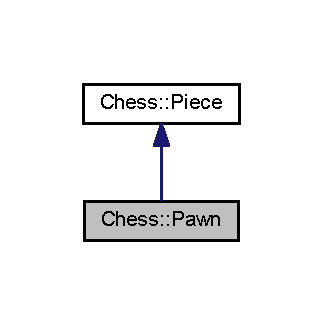
\includegraphics[width=155pt]{class_chess_1_1_pawn__coll__graph}
\end{center}
\end{figure}
\subsection*{Открытые члены}
\begin{DoxyCompactItemize}
\item 
\mbox{\Hypertarget{class_chess_1_1_pawn_ab4d91a80c4da18b87f44962ec68a03cb}\label{class_chess_1_1_pawn_ab4d91a80c4da18b87f44962ec68a03cb}} 
{\bfseries Pawn} (const Color color)
\item 
\mbox{\Hypertarget{class_chess_1_1_pawn_ae9725199f9bd4f3e37e4a05dd3f21bdc}\label{class_chess_1_1_pawn_ae9725199f9bd4f3e37e4a05dd3f21bdc}} 
bool {\bfseries check\+Move} (const \mbox{\hyperlink{class_chess_1_1_position}{Position}} \&pos\+\_\+current, const \mbox{\hyperlink{class_chess_1_1_position}{Position}} \&pos\+\_\+target, const std\+::array$<$ std\+::array$<$ \mbox{\hyperlink{class_chess_1_1_piece}{Piece}} $\ast$, B\+O\+A\+R\+D\+\_\+\+S\+I\+ZE $>$, B\+O\+A\+R\+D\+\_\+\+S\+I\+ZE $>$ \&chess\+\_\+board) const override
\item 
\mbox{\Hypertarget{class_chess_1_1_pawn_a839f5712501473ca3dc87ca8de2eec37}\label{class_chess_1_1_pawn_a839f5712501473ca3dc87ca8de2eec37}} 
\mbox{\hyperlink{class_chess_1_1_position}{Position}} $\ast$ {\bfseries return\+Available\+Moves} (int $\ast$list\+\_\+len, const \mbox{\hyperlink{class_chess_1_1_position}{Position}} \&pos\+\_\+current, const std\+::array$<$ std\+::array$<$ \mbox{\hyperlink{class_chess_1_1_piece}{Piece}} $\ast$, B\+O\+A\+R\+D\+\_\+\+S\+I\+ZE $>$, B\+O\+A\+R\+D\+\_\+\+S\+I\+ZE $>$ \&chess\+\_\+board) const override
\item 
\mbox{\Hypertarget{class_chess_1_1_pawn_a56116e06fc8e4a8236858bc6991b9bc0}\label{class_chess_1_1_pawn_a56116e06fc8e4a8236858bc6991b9bc0}} 
bool {\bfseries check\+Reachability} (const \mbox{\hyperlink{class_chess_1_1_position}{Position}} \&pos\+\_\+current, const \mbox{\hyperlink{class_chess_1_1_position}{Position}} \&pos\+\_\+target, const std\+::array$<$ std\+::array$<$ \mbox{\hyperlink{class_chess_1_1_piece}{Piece}} $\ast$, B\+O\+A\+R\+D\+\_\+\+S\+I\+ZE $>$, B\+O\+A\+R\+D\+\_\+\+S\+I\+ZE $>$ \&chess\+\_\+board) const override
\end{DoxyCompactItemize}
\subsection*{Дополнительные унаследованные члены}


Объявления и описания членов классов находятся в файлах\+:\begin{DoxyCompactItemize}
\item 
Pieces/pawn.\+h\item 
Pieces/pawn.\+cpp\end{DoxyCompactItemize}

\hypertarget{class_chess_1_1_piece}{}\section{Класс Chess\+:\+:Piece}
\label{class_chess_1_1_piece}\index{Chess\+::\+Piece@{Chess\+::\+Piece}}


Граф наследования\+:Chess\+:\+:Piece\+:\nopagebreak
\begin{figure}[H]
\begin{center}
\leavevmode
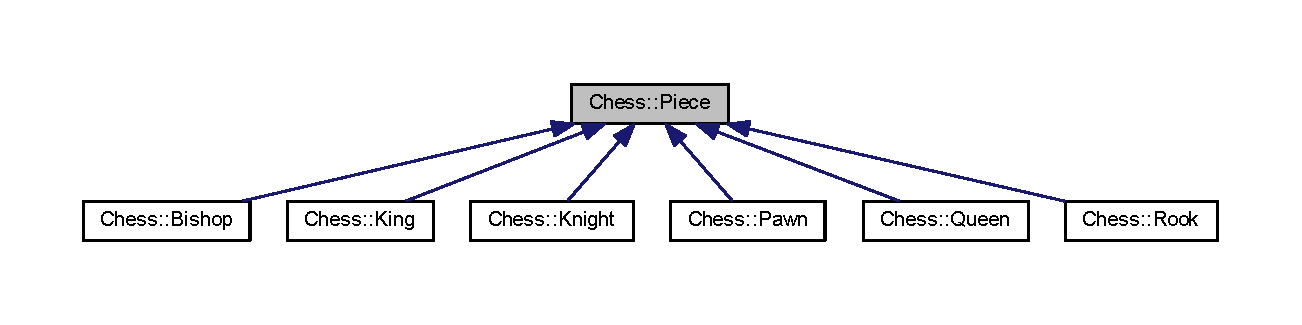
\includegraphics[width=350pt]{class_chess_1_1_piece__inherit__graph}
\end{center}
\end{figure}
\subsection*{Открытые типы}
\begin{DoxyCompactItemize}
\item 
\mbox{\Hypertarget{class_chess_1_1_piece_a65c480b6cb99b4e3732d6c14cf5f75e5}\label{class_chess_1_1_piece_a65c480b6cb99b4e3732d6c14cf5f75e5}} 
enum {\bfseries Color} \{ {\bfseries W\+H\+I\+TE} = 1, 
{\bfseries B\+L\+A\+CK}
 \}
\item 
\mbox{\Hypertarget{class_chess_1_1_piece_a691ee828590a8fe4a5aacc8669ed63c4}\label{class_chess_1_1_piece_a691ee828590a8fe4a5aacc8669ed63c4}} 
enum {\bfseries Name} \{ \newline
{\bfseries K\+I\+NG}, 
{\bfseries Q\+U\+E\+EN}, 
{\bfseries R\+O\+OK}, 
{\bfseries K\+N\+I\+G\+HT}, 
\newline
{\bfseries B\+I\+S\+H\+OP}, 
{\bfseries P\+A\+WN}
 \}
\end{DoxyCompactItemize}
\subsection*{Открытые члены}
\begin{DoxyCompactItemize}
\item 
\mbox{\Hypertarget{class_chess_1_1_piece_a641074d67cbc2f7d7290a8b721a57f16}\label{class_chess_1_1_piece_a641074d67cbc2f7d7290a8b721a57f16}} 
void {\bfseries set\+Color} (const Color color)
\item 
\mbox{\Hypertarget{class_chess_1_1_piece_abfc56a5956d7abf5e2b9765829b113ea}\label{class_chess_1_1_piece_abfc56a5956d7abf5e2b9765829b113ea}} 
void {\bfseries set\+Name} (const Name name)
\item 
\mbox{\Hypertarget{class_chess_1_1_piece_a234a31e7eb30f8f6112893fc97d2e270}\label{class_chess_1_1_piece_a234a31e7eb30f8f6112893fc97d2e270}} 
Color {\bfseries get\+Color} () const
\item 
\mbox{\Hypertarget{class_chess_1_1_piece_a145087e3b290d9a274dc301d3fe530ea}\label{class_chess_1_1_piece_a145087e3b290d9a274dc301d3fe530ea}} 
Name {\bfseries get\+Name} () const
\item 
\mbox{\Hypertarget{class_chess_1_1_piece_a2e94ad5b115beff701856fb947327b36}\label{class_chess_1_1_piece_a2e94ad5b115beff701856fb947327b36}} 
virtual bool {\bfseries check\+Move} (const \mbox{\hyperlink{class_chess_1_1_position}{Position}} \&pos\+\_\+current, const \mbox{\hyperlink{class_chess_1_1_position}{Position}} \&pos\+\_\+target, const std\+::array$<$ std\+::array$<$ \mbox{\hyperlink{class_chess_1_1_piece}{Piece}} $\ast$, B\+O\+A\+R\+D\+\_\+\+S\+I\+ZE $>$, B\+O\+A\+R\+D\+\_\+\+S\+I\+ZE $>$ \&chess\+\_\+board) const =0
\item 
\mbox{\Hypertarget{class_chess_1_1_piece_a6d4afbd864b16f2574cd5af30f961047}\label{class_chess_1_1_piece_a6d4afbd864b16f2574cd5af30f961047}} 
virtual \mbox{\hyperlink{class_chess_1_1_position}{Position}} $\ast$ {\bfseries return\+Available\+Moves} (int $\ast$list\+\_\+len, const \mbox{\hyperlink{class_chess_1_1_position}{Position}} \&pos\+\_\+current, const std\+::array$<$ std\+::array$<$ \mbox{\hyperlink{class_chess_1_1_piece}{Piece}} $\ast$, B\+O\+A\+R\+D\+\_\+\+S\+I\+ZE $>$, B\+O\+A\+R\+D\+\_\+\+S\+I\+ZE $>$ \&chess\+\_\+board) const =0
\item 
\mbox{\Hypertarget{class_chess_1_1_piece_a697016b0e460d10d45d0e75a8fdb82bf}\label{class_chess_1_1_piece_a697016b0e460d10d45d0e75a8fdb82bf}} 
virtual bool {\bfseries check\+Reachability} (const \mbox{\hyperlink{class_chess_1_1_position}{Position}} \&pos\+\_\+current, const \mbox{\hyperlink{class_chess_1_1_position}{Position}} \&pos\+\_\+target, const std\+::array$<$ std\+::array$<$ \mbox{\hyperlink{class_chess_1_1_piece}{Piece}} $\ast$, B\+O\+A\+R\+D\+\_\+\+S\+I\+ZE $>$, B\+O\+A\+R\+D\+\_\+\+S\+I\+ZE $>$ \&chess\+\_\+board) const =0
\end{DoxyCompactItemize}


Объявления и описания членов классов находятся в файлах\+:\begin{DoxyCompactItemize}
\item 
Pieces/piece.\+h\item 
Pieces/piece.\+cpp\end{DoxyCompactItemize}

\hypertarget{class_chess_1_1_player}{}\section{Класс Chess\+:\+:Player}
\label{class_chess_1_1_player}\index{Chess\+::\+Player@{Chess\+::\+Player}}
\subsection*{Открытые члены}
\begin{DoxyCompactItemize}
\item 
\mbox{\Hypertarget{class_chess_1_1_player_a3ea018efe28264e87808c82f97d71c5e}\label{class_chess_1_1_player_a3ea018efe28264e87808c82f97d71c5e}} 
{\bfseries Player} (const char $\ast$name, const long long rating=0)
\item 
\mbox{\Hypertarget{class_chess_1_1_player_a6e2b81aecdac98135da1c05a231cc4bc}\label{class_chess_1_1_player_a6e2b81aecdac98135da1c05a231cc4bc}} 
void {\bfseries set\+Name} (const char $\ast$name)
\item 
\mbox{\Hypertarget{class_chess_1_1_player_ac02bf8b66e1d1e476fcee572bc91ac85}\label{class_chess_1_1_player_ac02bf8b66e1d1e476fcee572bc91ac85}} 
const char $\ast$ {\bfseries get\+Name} () const
\item 
\mbox{\Hypertarget{class_chess_1_1_player_ac4891c8757a4feb6d0d0aac8d127f163}\label{class_chess_1_1_player_ac4891c8757a4feb6d0d0aac8d127f163}} 
void {\bfseries set\+Rating} (const long long rating)
\item 
\mbox{\Hypertarget{class_chess_1_1_player_ae30b121959ec3088d9c9c514faba72ae}\label{class_chess_1_1_player_ae30b121959ec3088d9c9c514faba72ae}} 
\mbox{\hyperlink{class_chess_1_1_player}{Player}} \& {\bfseries add\+Rating} (const long long value)
\item 
\mbox{\Hypertarget{class_chess_1_1_player_a0dfde9f2462faa0da76a54bca4b56fbc}\label{class_chess_1_1_player_a0dfde9f2462faa0da76a54bca4b56fbc}} 
\mbox{\hyperlink{class_chess_1_1_player}{Player}} \& {\bfseries reduce\+Rating} (const long long value)
\item 
\mbox{\Hypertarget{class_chess_1_1_player_a183ccce7828e84e2950078729f8d7fed}\label{class_chess_1_1_player_a183ccce7828e84e2950078729f8d7fed}} 
long long {\bfseries get\+Rating} () const
\end{DoxyCompactItemize}
\subsection*{Друзья}
\begin{DoxyCompactItemize}
\item 
\mbox{\Hypertarget{class_chess_1_1_player_aeb31617a48e2242cbb1a0e8be2cb1544}\label{class_chess_1_1_player_aeb31617a48e2242cbb1a0e8be2cb1544}} 
std\+::ostream \& {\bfseries operator$<$$<$} (std\+::ostream \&os, const \mbox{\hyperlink{class_chess_1_1_player}{Player}} \&player)
\end{DoxyCompactItemize}


Объявления и описания членов классов находятся в файлах\+:\begin{DoxyCompactItemize}
\item 
player.\+h\item 
player.\+cpp\end{DoxyCompactItemize}

\hypertarget{class_chess_1_1_position}{}\section{Класс Chess\+:\+:Position}
\label{class_chess_1_1_position}\index{Chess\+::\+Position@{Chess\+::\+Position}}
\subsection*{Открытые члены}
\begin{DoxyCompactItemize}
\item 
\mbox{\Hypertarget{class_chess_1_1_position_a8ec2fb21251eb9cd336530543ffd530f}\label{class_chess_1_1_position_a8ec2fb21251eb9cd336530543ffd530f}} 
{\bfseries Position} (const int x, const int y)
\item 
\mbox{\Hypertarget{class_chess_1_1_position_acf77554adfe13e96ad10a76e96d73a5d}\label{class_chess_1_1_position_acf77554adfe13e96ad10a76e96d73a5d}} 
int {\bfseries X} () const
\item 
\mbox{\Hypertarget{class_chess_1_1_position_a0cef56f45ccf302a87485ef3467a5e34}\label{class_chess_1_1_position_a0cef56f45ccf302a87485ef3467a5e34}} 
int {\bfseries Y} () const
\item 
\mbox{\Hypertarget{class_chess_1_1_position_a47e4bcc27c98e7a718ca91b6e310e339}\label{class_chess_1_1_position_a47e4bcc27c98e7a718ca91b6e310e339}} 
void {\bfseries X} (const int x)
\item 
\mbox{\Hypertarget{class_chess_1_1_position_af0537ad95983f9423998de1239358fab}\label{class_chess_1_1_position_af0537ad95983f9423998de1239358fab}} 
void {\bfseries Y} (const int y)
\item 
\mbox{\Hypertarget{class_chess_1_1_position_a660ce84d78c1694e1ba8310b694ea820}\label{class_chess_1_1_position_a660ce84d78c1694e1ba8310b694ea820}} 
const \mbox{\hyperlink{class_chess_1_1_position}{Position}} {\bfseries operator+} (const \mbox{\hyperlink{class_chess_1_1_position}{Position}} \&b) const
\item 
\mbox{\Hypertarget{class_chess_1_1_position_aa67a11d7efa1a12af19b5addc1cd089e}\label{class_chess_1_1_position_aa67a11d7efa1a12af19b5addc1cd089e}} 
\mbox{\hyperlink{class_chess_1_1_position}{Position}} \& {\bfseries operator+=} (const \mbox{\hyperlink{class_chess_1_1_position}{Position}} \&b)
\item 
\mbox{\Hypertarget{class_chess_1_1_position_a4b143d59104de22020111e8f2b9cc3a3}\label{class_chess_1_1_position_a4b143d59104de22020111e8f2b9cc3a3}} 
bool {\bfseries operator==} (const \mbox{\hyperlink{class_chess_1_1_position}{Position}} \&b) const
\end{DoxyCompactItemize}


Объявления и описания членов классов находятся в файлах\+:\begin{DoxyCompactItemize}
\item 
Pieces/position.\+h\item 
Pieces/position.\+cpp\end{DoxyCompactItemize}

\hypertarget{class_chess_1_1_queen}{}\section{Класс Chess\+:\+:Queen}
\label{class_chess_1_1_queen}\index{Chess\+::\+Queen@{Chess\+::\+Queen}}


Граф наследования\+:Chess\+:\+:Queen\+:\nopagebreak
\begin{figure}[H]
\begin{center}
\leavevmode
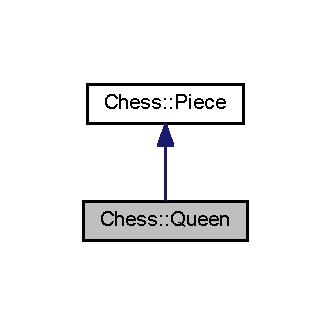
\includegraphics[width=159pt]{class_chess_1_1_queen__inherit__graph}
\end{center}
\end{figure}


Граф связей класса Chess\+:\+:Queen\+:\nopagebreak
\begin{figure}[H]
\begin{center}
\leavevmode
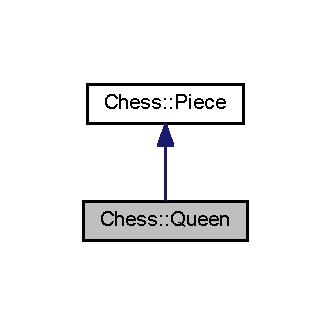
\includegraphics[width=159pt]{class_chess_1_1_queen__coll__graph}
\end{center}
\end{figure}
\subsection*{Открытые члены}
\begin{DoxyCompactItemize}
\item 
\mbox{\Hypertarget{class_chess_1_1_queen_a60311431cf43c98d3d47ac2f45f222ef}\label{class_chess_1_1_queen_a60311431cf43c98d3d47ac2f45f222ef}} 
{\bfseries Queen} (const Color color)
\item 
\mbox{\Hypertarget{class_chess_1_1_queen_a3b208172bb8bc1fbcda3c232b1c5a612}\label{class_chess_1_1_queen_a3b208172bb8bc1fbcda3c232b1c5a612}} 
bool {\bfseries check\+Move} (const \mbox{\hyperlink{class_chess_1_1_position}{Position}} \&pos\+\_\+current, const \mbox{\hyperlink{class_chess_1_1_position}{Position}} \&pos\+\_\+target, const std\+::array$<$ std\+::array$<$ \mbox{\hyperlink{class_chess_1_1_piece}{Piece}} $\ast$, B\+O\+A\+R\+D\+\_\+\+S\+I\+ZE $>$, B\+O\+A\+R\+D\+\_\+\+S\+I\+ZE $>$ \&chess\+\_\+board) const override
\item 
\mbox{\Hypertarget{class_chess_1_1_queen_ab38744d01eac33fce5c917ee726bb323}\label{class_chess_1_1_queen_ab38744d01eac33fce5c917ee726bb323}} 
\mbox{\hyperlink{class_chess_1_1_position}{Position}} $\ast$ {\bfseries return\+Available\+Moves} (int $\ast$list\+\_\+len, const \mbox{\hyperlink{class_chess_1_1_position}{Position}} \&pos\+\_\+current, const std\+::array$<$ std\+::array$<$ \mbox{\hyperlink{class_chess_1_1_piece}{Piece}} $\ast$, B\+O\+A\+R\+D\+\_\+\+S\+I\+ZE $>$, B\+O\+A\+R\+D\+\_\+\+S\+I\+ZE $>$ \&chess\+\_\+board) const override
\item 
\mbox{\Hypertarget{class_chess_1_1_queen_af4cfcec4022fc26e99b89559ca3d6bc7}\label{class_chess_1_1_queen_af4cfcec4022fc26e99b89559ca3d6bc7}} 
bool {\bfseries check\+Reachability} (const \mbox{\hyperlink{class_chess_1_1_position}{Position}} \&pos\+\_\+current, const \mbox{\hyperlink{class_chess_1_1_position}{Position}} \&pos\+\_\+target, const std\+::array$<$ std\+::array$<$ \mbox{\hyperlink{class_chess_1_1_piece}{Piece}} $\ast$, B\+O\+A\+R\+D\+\_\+\+S\+I\+ZE $>$, B\+O\+A\+R\+D\+\_\+\+S\+I\+ZE $>$ \&chess\+\_\+board) const override
\end{DoxyCompactItemize}
\subsection*{Дополнительные унаследованные члены}


Объявления и описания членов классов находятся в файлах\+:\begin{DoxyCompactItemize}
\item 
Pieces/queen.\+h\item 
Pieces/queen.\+cpp\end{DoxyCompactItemize}

\hypertarget{class_chess_1_1_rook}{}\section{Класс Chess\+:\+:Rook}
\label{class_chess_1_1_rook}\index{Chess\+::\+Rook@{Chess\+::\+Rook}}


Граф наследования\+:Chess\+:\+:Rook\+:\nopagebreak
\begin{figure}[H]
\begin{center}
\leavevmode
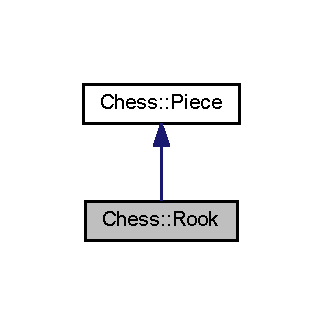
\includegraphics[width=155pt]{class_chess_1_1_rook__inherit__graph}
\end{center}
\end{figure}


Граф связей класса Chess\+:\+:Rook\+:\nopagebreak
\begin{figure}[H]
\begin{center}
\leavevmode
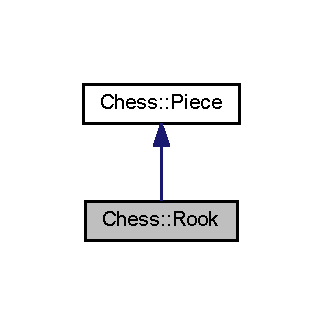
\includegraphics[width=155pt]{class_chess_1_1_rook__coll__graph}
\end{center}
\end{figure}
\subsection*{Открытые члены}
\begin{DoxyCompactItemize}
\item 
\mbox{\Hypertarget{class_chess_1_1_rook_a6ea7f044b41cf7463f9e48381631ab38}\label{class_chess_1_1_rook_a6ea7f044b41cf7463f9e48381631ab38}} 
{\bfseries Rook} (const Color color)
\item 
\mbox{\Hypertarget{class_chess_1_1_rook_a5c99e8a5076f9bf139f7b45c33989483}\label{class_chess_1_1_rook_a5c99e8a5076f9bf139f7b45c33989483}} 
bool {\bfseries check\+Move} (const \mbox{\hyperlink{class_chess_1_1_position}{Position}} \&pos\+\_\+current, const \mbox{\hyperlink{class_chess_1_1_position}{Position}} \&pos\+\_\+target, const std\+::array$<$ std\+::array$<$ \mbox{\hyperlink{class_chess_1_1_piece}{Piece}} $\ast$, B\+O\+A\+R\+D\+\_\+\+S\+I\+ZE $>$, B\+O\+A\+R\+D\+\_\+\+S\+I\+ZE $>$ \&chess\+\_\+board) const override
\item 
\mbox{\Hypertarget{class_chess_1_1_rook_aeb9a352eea0c12eafb3b65aa9ae8b3ab}\label{class_chess_1_1_rook_aeb9a352eea0c12eafb3b65aa9ae8b3ab}} 
\mbox{\hyperlink{class_chess_1_1_position}{Position}} $\ast$ {\bfseries return\+Available\+Moves} (int $\ast$list\+\_\+len, const \mbox{\hyperlink{class_chess_1_1_position}{Position}} \&pos\+\_\+current, const std\+::array$<$ std\+::array$<$ \mbox{\hyperlink{class_chess_1_1_piece}{Piece}} $\ast$, B\+O\+A\+R\+D\+\_\+\+S\+I\+ZE $>$, B\+O\+A\+R\+D\+\_\+\+S\+I\+ZE $>$ \&chess\+\_\+board) const override
\item 
\mbox{\Hypertarget{class_chess_1_1_rook_a5ae20056849a9a1dc5fc25f731974c75}\label{class_chess_1_1_rook_a5ae20056849a9a1dc5fc25f731974c75}} 
bool {\bfseries check\+Reachability} (const \mbox{\hyperlink{class_chess_1_1_position}{Position}} \&pos\+\_\+current, const \mbox{\hyperlink{class_chess_1_1_position}{Position}} \&pos\+\_\+target, const std\+::array$<$ std\+::array$<$ \mbox{\hyperlink{class_chess_1_1_piece}{Piece}} $\ast$, B\+O\+A\+R\+D\+\_\+\+S\+I\+ZE $>$, B\+O\+A\+R\+D\+\_\+\+S\+I\+ZE $>$ \&chess\+\_\+board) const override
\end{DoxyCompactItemize}
\subsection*{Дополнительные унаследованные члены}


Объявления и описания членов классов находятся в файлах\+:\begin{DoxyCompactItemize}
\item 
Pieces/rook.\+h\item 
Pieces/rook.\+cpp\end{DoxyCompactItemize}

%--- End generated contents ---

% Index
\backmatter
\newpage
\phantomsection
\clearemptydoublepage
\addcontentsline{toc}{chapter}{Алфавитный указатель}
\printindex

\end{document}
